% MRA tree schematic showing receptive field limitation (Figure 4)
% Compile: pdflatex fig4_tree_schematic.tex
\documentclass[tikz,border=5pt]{standalone}
\usepackage{tikz}
\usetikzlibrary{positioning, arrows.meta, decorations.pathreplacing}

\begin{document}
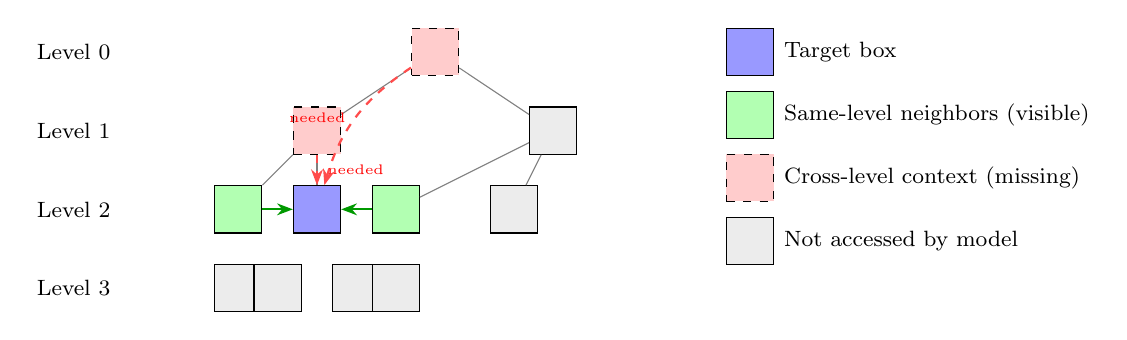
\begin{tikzpicture}[
    box/.style={draw, minimum size=0.6cm, inner sep=0pt},
    seen/.style={box, fill=green!30},
    center/.style={box, fill=blue!40},
    unseen/.style={box, fill=gray!15},
    needed/.style={box, fill=red!20, dashed},
    arrow/.style={-{Stealth[length=2mm]}, thick},
    brace/.style={decorate, decoration={brace, amplitude=5pt}},
]

% Level labels
\foreach \y/\lbl in {4/Level 0, 3/Level 1, 2/Level 2, 1/Level 3} {
    \node[font=\footnotesize, anchor=east] at (-1, \y) {\lbl};
}

% Level 0 (root)
\node[needed] (r0) at (3, 4) {};

% Level 1
\node[needed] (l1a) at (1.5, 3) {};
\node[unseen] (l1b) at (4.5, 3) {};

% Level 2 (target level)
\node[seen] (l2a) at (0.5, 2) {};
\node[center] (l2b) at (1.5, 2) {};
\node[seen] (l2c) at (2.5, 2) {};
\node[unseen] (l2d) at (4, 2) {};

% Level 3 (children)
\node[unseen] (l3a) at (0.5, 1) {};
\node[unseen] (l3b) at (1, 1) {};
\node[unseen] (l3c) at (2, 1) {};
\node[unseen] (l3d) at (2.5, 1) {};

% Parent-child edges
\draw[gray, thin] (r0) -- (l1a);
\draw[gray, thin] (r0) -- (l1b);
\draw[gray, thin] (l1a) -- (l2a);
\draw[gray, thin] (l1a) -- (l2b);
\draw[gray, thin] (l1b) -- (l2c);
\draw[gray, thin] (l1b) -- (l2d);

% What model sees (same-level neighbors)
\draw[arrow, green!60!black] (l2a) -- (l2b);
\draw[arrow, green!60!black] (l2c) -- (l2b);

% What model NEEDS (cross-level)
\draw[arrow, red!70, dashed, thick] (l1a) -- node[right, font=\tiny, text=red] {needed} (l2b);
\draw[arrow, red!70, dashed, thick] (r0) to[bend right=20] node[left, font=\tiny, text=red] {needed} (l2b);

% Legend
\node[center, label=right:{\footnotesize Target box}] at (7, 4) {};
\node[seen, label=right:{\footnotesize Same-level neighbors (visible)}] at (7, 3.2) {};
\node[needed, label=right:{\footnotesize Cross-level context (missing)}] at (7, 2.4) {};
\node[unseen, label=right:{\footnotesize Not accessed by model}] at (7, 1.6) {};

\end{tikzpicture}
\end{document}
